\subsection{Needham Schroeder Symmetric Key}

In questa sezione vedremo come è possibile modellare attraverso i diagrammi object diagram dello standard UML il protocollo di sicurezza a chiave simmetrica proposto da Needham e Schroeder:
\begin{lstlisting}[mathescape]
    1. $A \rightarrow S : A, B, N_a$
    2. $S \rightarrow A : \{N_a, K_{ab}, B, \{K_{ab}, A\}_{K_{bs}}\}_{K_{as}}$
    3. $A \rightarrow B : \{K_{ab}, A\}_{K_{bs}}$
    4. $B \rightarrow A : \{N_b\}_{K_{as}}$
    5. $A \rightarrow B : \{N_b-1\}_{K_{as}}$
\end{lstlisting} 

\noindent Nelle Figure seguenti avremo i seguenti partecipanti al protocollo: l'agente \texttt{Initiator} che vuole iniziare la comunicazione con l'agente \texttt{Recipient} e richiede la password per la comunicazione al server \texttt{S}.\\
Inoltre la chiave simmetrica viene rappresentata in questo modo \texttt{SK($a$,$b$)}, dove $a$ e $b$ indicano l'identità degli agenti proprietari della chiave.\\
\newpage
\begin{figure}[h!] 
    \centering 
    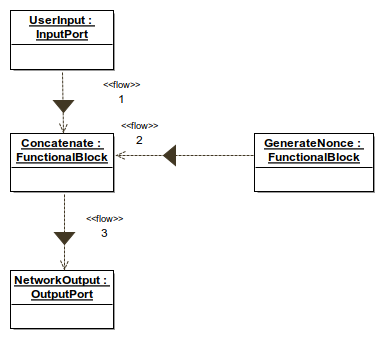
\includegraphics[scale=0.6]{../img/NSSK/First_message(toServer)_Object_diagram.png} 
    \begin{lstlisting}[frame=single, mathescape, basicstyle=\footnotesize]
        1. $<i.name, r.name>$
        2. $<i.nonce>$
        3. $<i.name, r.name, i.nonce>$
    \end{lstlisting}
    \caption{$A \rightarrow B : A, B, N_a$} 
\end{figure}
\noindent Nell'oggetto UserInput il sistema che andrà ad implementare il protocollo riceve il nome ($r.name$) dell'agente \texttt{Recipient}, l'oggetto GenerateNonce genera un nuovo Nonce e l'oggetto Concatenate prepara il pacchetto da mandare al server \texttt{S} attraverso l'oggetto NetworkOPort, composto da $i.name, r.name, i.nonce$, ovvero dai nomi dei partecipanti al protocollo e il nonce per assicurarsi che la comunicazione sia fresh.
\newpage
\begin{figure}[h!] 
    \centering 
    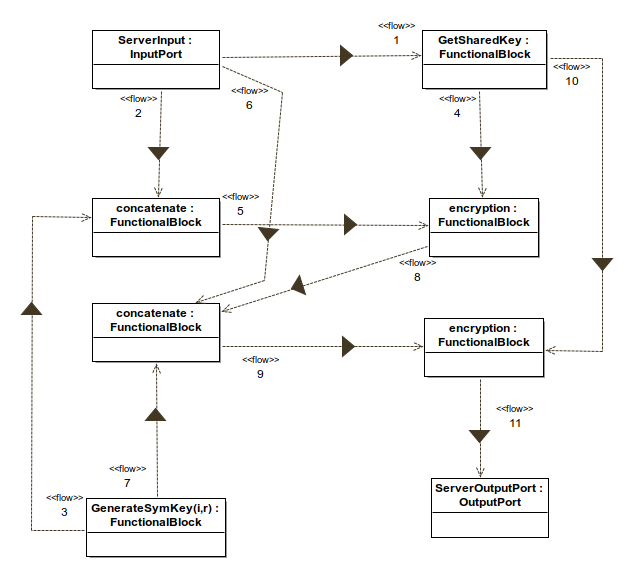
\includegraphics[scale=0.5]{../img/NSSK/Second_Message(fromServer).png} 
    \begin{lstlisting}[frame=single, mathescape, basicstyle=\footnotesize]
        1. $<i.name,r.name>$
        2. $<i.name>$
        3. $<SK(i,r)>$
        4. $<SK(s,r)>$
        5. $<i.name, SK(i,r)>$
        6. $<r.name, i.nonce>$
        7. $<SK(i,r)>$
        8. $<\{i.name; SK(i,r)\}\_SK(r,s)>$
        9. $<i.nonce, r.name, SK(i,r), \{i.name,SymKey(i,r)\}\_SK(r,s)\}>$
        10. $<SK(s,r)>$
        11. $<\{i.nonce, r.name, SK(i,r), \{i.name,SK(i,r)\}\_SK(rs)\}\}\_SK(i,s)>$
    \end{lstlisting}
    \caption{$S \rightarrow A : \{N_a, K_{ab}, B, \{K_{ab}, A\}_{K_{bs}}\}_{K_{as}}$} 
\end{figure}
\noindent Una volta ricevuto il pacchetto, il server \texttt{S} provvede alla generazione della chiave simmetrica (\texttt{SK($i$,$r$)}) per la comunicazione tra \texttt{Initiator} e \texttt{Recipient} utilizzando l'oggetto GenerateSymKey($i$,$r$), passando a quest'ultimo i nomi $i.name, r.name$ dei partecipanti.\\ 
A questo punto, fornendo sempre come input i nomi dei partecipanti all'oggetto GetSharedKey, ottiene le chiavi simmetriche precedentemente condivise tra lui e ogni agente partecipante (\texttt{SK($i$,$s$)} e \texttt{SK($r$,$s$)}).\\ 
La chiave \texttt{SK($r$,$s$)} verrà utilizzata dall'oggetto encryption dopo aver preparato con l'oggetto Concatenate il pacchetto per l'agente \texttt{Recipient}, questo pacchetto a sua volta verrà inserito da un altro oggetto Concatenate nel pacchetto per l'agente \texttt{Initiator} e il tutto verrà cifrato da un altro oggetto encryption con la chiave \texttt{SK($i$,$s$)}. Il pacchetto risultante da queste operazioni verrà spedito all'agente \texttt{Initiator} attraverso l'oggetto ServerOutputPort.\\

\begin{figure}[h!] 
    \centering 
    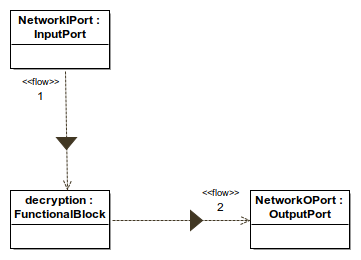
\includegraphics[scale=0.6]{../img/NSSK/FirstMessage.png} 
    \begin{lstlisting}[frame=single, mathescape, basicstyle=\footnotesize]
        1. $<\{i.nonce, r.name, SK(i,r), \{i.name,SK(i,r)\}\_SK(r,s)\}\_SK(i,s)>$
        2. $<\{i.name,SK(i,r)\}\_SK(r,s)>$
    \end{lstlisting}
    \caption{$A \rightarrow B : \{K_{ab}, A\}_{K_{bs}}$} 
\end{figure}
\noindent L'agente \texttt{Initiator} riceve il pacchetto attraverso l'oggetto NetworkIPort e utilizza l'oggetto di decryption con la chiave simmetrica \texttt{SK($i$,$s$)} per estrarre il pacchetto da inoltrare all'agente \texttt{Recipient} attraverso l'oggetto NetworkOPort.\\
\begin{figure}[h!] 
    \centering 
    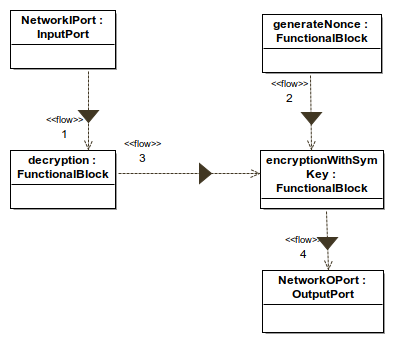
\includegraphics[scale=0.59]{../img/NSSK/SecondMessage.png} 
    \begin{lstlisting}[frame=single, mathescape, basicstyle=\footnotesize]
        1. $<\{i.name,SK(i,r)\}\_SK(r,s)>$
        2. $<r.nonce>$
        3. $<SK(i,s)>$
        4. $<\{r.nonce\}\_SK(i,r)>$
    \end{lstlisting}
    \caption{$B \rightarrow A : \{N_b\}_{K_{as}}$} 
\end{figure}
\newpage
\noindent L'agente \texttt{Recipient} riceve il pacchetto attraverso l'oggetto NetworkIPort, lo decifra con l'oggetto decryption utilizzando la chiave \texttt{SK($r$,$s$)} ed estrae la chiave \texttt{SK($i$,$r$)}.\\ 
\texttt{SK($i$,$r$)} verrà utilizzata dall'oggetto encryptionWithSymKey per cifrare un nuovo pacchetto contenente il Nonce generato dall'oggetto generateNonce.\\ 
Infine l'agente \texttt{Recipient} spedisce il pacchetto all'agente \texttt{Initiator} utilizzando l'oggetto NetworkOPort.\\
\begin{figure}[h!] 
    \centering 
    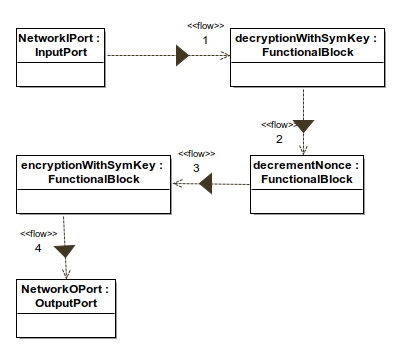
\includegraphics[scale=0.6]{../img/NSSK/ThirdMessage.png} 
    \begin{lstlisting}[frame=single, mathescape, basicstyle=\footnotesize]
        1. $<{r.nonce}\_SK(i,r)>$
        2. $<r.nonce>$
        3. $<r.nonce-1>$
        4. $<\{r.nonce-1\}\_SK(i,r)>$
    \end{lstlisting}
    \caption{$A \rightarrow B : \{N_b-1\}_{K_{as}}$} 
\end{figure}\\
\noindent Nell'ultima fase del protocollo, l'agente \texttt{Initiator} riceve dall'oggetto NetworkIPort il pacchetto contenente il Nonce, lo decifra con l'oggetto decryptionWithSymKey utilizzando la chiave \texttt{SK($i$,$r$)}, utilizza l'oggetto decrementNonce per sottrarre 1 al Nonce inviato dall'agente \texttt{Recipient} e cifra il risultato con l'oggetto encryptionWithSymKey utilizzando la chiave \texttt{SK($i$,$r$)}.\\
Il pacchetto risultante viene spedito all'agente \texttt{Recipient} attraverso l'oggetto NetworkOPort.\\

\newpage
\subsubsection*{Tool di verifica}
Dopo aver modellato il protocollo ed estratto il file .xmi visibile nel Listing \ref{lst:ns1}\footnote{\label{note:a}Listing in Appendice \ref{app:ns}}, si utilizza il tool di conversione per ottenere il file delle strutture Listing \ref{lst:ns2}\textsuperscript{\ref{note:a}}.\\
Sempre con il tool di conversione ricaviamo il seguente file da utilizzare come input a VerifPal:

\lstinputlisting[label={lst:nssk.vp},caption={File nssk.vp},language=vp, breaklines= true]{../code/verifpal/nssk.vp}

\noindent In questo esempio vengono verificate la confidenzialità della chiave \textbf{k\_ir}, la confidenzialità del Nonce \textbf{n\_r\_minus\_one} e l'autenticazione dell'ultimo pacchetto del protocollo.\\
Nel Listing \ref{lst:ns3}\footnote{Listing in Appendice \ref{app:ns}} troviamo il risultato dell'analisi.\\
Come dimostrato da Denning-Sacco in \cite{DS81} il protocollo è soggetto ad attacchi di tipo reply attack, se l'attaccante viene a conoscenza della chiave condivisa tra i due principal.\\
In questo modello l'attaccante in qualche modo riesce ad ottenere la chiave e di conseguenza i risultati della verifica diranno che la chiave non è confidenziale, come non è confidenziale il Nonce \textbf{n\_r\_minus\_one}, oltre al fatto che può essere lo stesso attaccante ad inviare il pacchetto \textbf{e\_n\_r\_minus\_one} al principal \texttt{Recipient} fingendosi il principal Initiator, violando l'autenticazione.\\
Per completezza in Appendice \ref{app:ns} vengono riportate la modellazione del protocollo in Applied Pi Calculus nel Listing \ref{lst:ns4} e i risultati ottenuti con ProVerif nel Listing \ref{lst:ns5}, i quali rispecchiano i risultati ottenuti con VerifPal.

\subsubsection*{Osservazioni}
L'esecuzione del modello di questo protocollo consiste in una sola sessione dove l'attaccante è a conoscenza della chiave simmetrica tra i due principal, questo definisce uno scenario ben specifico infatti non è sempre vero che l'attaccante riesca ad ottenere la chiave simmetrica.\\
Con questa premessa si capisce come l'utilizzatore del tool per la verifica dovrebbe avere ben chiaro lo scenario in cui modellare il protocollo e allo stesso tempo dovrebbe avere almeno l'intuizione per capire sotto quali condizioni il protocollo può essere violato, per poterlo testare in diversi scenari.\\
Facendo vari tipi di verifiche sul protocollo è infatti emerso un limite dei verificatori automatici, ovvero il fatto di dover modellare il protocollo in uno specifico scenario per verificare la presenza di un determinato tipo di attacco, eventualmente già noto.\\ 
Per diversificare gli scenari, l'utilizzatore del tool può aumentare il numero di sessioni del protocollo, oppure fornire ad un certo punto dell'esecuzione del protocollo delle informazioni all'attaccante, come abbiamo visto in questo caso.\\
Queste tecniche consentono al tool di verifica di fornire delle risposte valide ai quesiti, evitando la non terminazione o risposte del tipo ``Non lo so''. 
